\begin{designation}
	Далее мы начинаем активно пользоваться довольно популярным обозначением значения функции в функциональном анализе (особенно будет актуально при рассмотрении линейных отображений):
	\[
		fx := f(x)
	\]
\end{designation}

\begin{definition}
	Пусть $X$ --- полное метрическое пространство. Тогда отображение $f \colon X \to X$ называется \textit{сжимающим}, если выполнено утверждение:
	\[
		\exists \alpha \in (0; 1) \such \forall x, y \in X\ \ \rho(f(x), f(y)) \le \alpha\rho(x, y)
	\]
\end{definition}

\begin{theorem} (Банаха, 1922г.)
	Пусть $X$ --- полное метрическое пространство, $f \colon X \to X$ --- сжимающее отображение. Тогда существует и единственна неподвижная точка отображения $f$.
\end{theorem}

\begin{proof}
	Сразу отметим, что сжимающее отображение обязано быть непрерывным. Действительно, если $\{y_n\}_{n = 1}^\infty \subseteq X$ сходится к $y \in X$, то верна оценка:
	\[
		\rho(fy, fy_n) \le \alpha\rho(y, y_n) \xrightarrow[n \to \infty]{} 0
	\]
	Что по определению означает непрерывность $f$. Теперь мы готовы доказывать основной факт теоремы:
	\begin{itemize}
		\item Существование. Пусть $x_0 \in X$. Рассмотрим последовательность $\{x_n\}_{n = 0}^\infty$, называемую \textit{орбитой} $x_0$ и полученную по правилу $x_{n + 1} = fx_n$. Покажем, что эта последовательность сходится. Это эквивалентно её фундаментальности:
		\begin{multline*}
			\forall n, m \in \N\ \ \rho(x_{n + m}, x_n) \le \rho(x_{n + m}, x_{n + m - 1}) + \ldots + \rho(x_{n + 1}, x_n) \le
			\\
			\rho(x_1, x_0)(\alpha^{n + m - 1} + \ldots + \alpha^n) < \rho(x_1, x_0) \frac{\alpha^n}{1 - \alpha}
		\end{multline*}
		За счёт этого неравенства, фундаментальность показывается уже тривиально. Осталось обозначить $x := \lim_{n \to \infty} x_n$ и сделать следующее забавное наблюдение:
		\[
			fx = \lim_{n \to \infty} fx_n = \lim_{n \to \infty} x_{n + 1} = x
		\]
		
		\item Единственность. Пусть $x, y \in X$ --- две неподвижные точки. Тогда, в силу свойств $f$ верно неравенство:
		\[
			\rho(x, y) = \rho(fx, fy) \le \alpha\rho(x, y)
		\]
		Так как $\alpha \in (0; 1)$, то такое возможно тогда и только тогда, когда $\rho(x, y) = 0$, а в силу определения метрики это гарантирует равенство $x = y$.
	\end{itemize}
\end{proof}

\begin{definition} (не по лектору)
	Пусть $X, Y$ --- метрические пространства. Тогда \textit{изометрией} называется отображение $f \colon X \to Y$, которое \textit{сохраняет (или, говорят, уважает)} метрики пространств:
	\[
		\forall x_1, x_2 \in X\ \ \rho_X(x_1, x_2) = \rho_Y(f(x_1), f(x_2))
	\]
\end{definition}

\begin{theorem} (Хаусдорфа, без доказательства)
	Пусть $X$ --- неполное метрическое пространство. Тогда существует и единственно (с точностью до изометрии) полное метрическое пространство $Y$ такое, что существует изометрия $\pi \colon X \to Y$ со следующим свойством:
	\[
		\cl(\pi X) = Y
	\]
\end{theorem}

\begin{note}
	Можно вспомнить, как из $\Q$ строится $\R$ --- фактически добавляются все возможные пределы. Так и тут основная идея состоит в том, чтобы разрешить всем сходящимся последовательностям из $X$ сходиться, нужно произвести пополнение пространства $X$ этими пределами.
\end{note}

\begin{exercise}
	Пусть $X_1$ и $X_2$ --- гомеоморфные метрические пространства. Если $X_1$ полное, то верно ли, что и $X_2$ такое?
\end{exercise}

\begin{solution}
	Нет, неверно. Достаточно посмотреть изоморфизм между половиной окружности с выколотыми точками и прямой
\end{solution}

\section{Компактные топологические и метрические пространства}

\begin{definition}
	Топологическое пространство $X$ называется \textit{компактным}, если для любого открытого покрытия $X$ можно выделить конечное подпокрытие:
	\[
		\forall \gA \such \bigcup_{\alpha \in \gA} G_\alpha \supseteq X \Lora \exists \gM, |\gM| < \infty\ \bigcup_{\alpha \in \gM} G_\alpha \supseteq X
	\]
\end{definition}

\begin{definition}
	Пусть $X$ --- произвольное множество. Произвольный набор множеств $\{Y_\alpha\}_{\alpha \in \gA} \subseteq 2^X$ называется \textit{центрированной системой множеств}, если любая конечная подсистема из этих множеств имеет непустое пересечение.
\end{definition}

\begin{theorem}
	Топологическое пространство $X$ является компактным тогда и только тогда, когда любая центрированная система замкнутых множеств имеет непустое пересечение (то есть пересечение всех множеств системы непусто).
\end{theorem}

\begin{proof}~
	\begin{itemize}
		\item[$\Ra$] Пусть $\{F_\alpha\}_{\alpha \in \gA}$ --- центрированная система замкнутых множеств. Введём $G_\alpha := X \bs F_\alpha$ и заметим, что из этого набора нельзя выделить конечное покрытие $X$. Действительно, предположим противное: $\bigcup_{k = 1}^n G_k = X$. Но тогда:
		\[
			\bigcup_{k = 1}^n X \bs F_k = X \bs \ps{\bigcap_{k = 1}^n F_k} = X
		\]
		Последнее равенство является противоречием, ведь $F_k$ были взяты из центрированной системы множеств.
		
		Так как $X$ по условию было компактом, то $\{G_\alpha\}_{\alpha \in \gA}$ не является покрытием $X$. Коль скоро это так, мы доказали требуемое:
		\[
			\bigcap_{\alpha \in \gA} F_\alpha = \bigcap_{\alpha \in \gA} X \bs G_\alpha = X \bs \bigcup_{\alpha \in \gA} G_\alpha \neq \emptyset
		\]
		
		\item[$\La$] Пусть $X = \bigcup_{\alpha \in \gA} G_\alpha$ --- произвольное покрытие открытыми множествами. Введём $F_\alpha = X \bs G_\alpha$, тогда $\{F_\alpha\}_{\alpha \in \gA}$ не образуют центрированную систему замкнутых множеств (иначе тривиальное противоречие по уже сказанному выше). Стало быть, существует конечная подсистема $F_k$ с пустым пересечением:
		\[
			\bigcap_{k = 1}^n F_k = \emptyset = \bigcap_{k = 1}^n X \bs G_k = X \bs \bigcup_{k = 1}^n G_k \Lolra X = \bigcup_{k = 1}^n G_k
		\]
	\end{itemize}
\end{proof}

\begin{exercise}
	Компактность топологических пространств сохраняется при непрерывном отображении
\end{exercise}

\begin{definition}
	Множество $Y$ в метрическом пространстве $X$ называется \textit{вполне ограниченным}, если для любого $\eps > 0$ существует конечное множество $\{a_k\}_{k = 1}^n \subseteq X$ такое, что выполнено условие:
	\[
		\forall y \in Y\ \ \min_{k \in \range{1}{n}} \rho(y, a_k) < \eps
	\]
	При этом множество $\{a_k\}_{k = 1}^n$ называется \textit{$\eps$-сетью}.
\end{definition}

\begin{note}
	Для $\R^n$ с любой метрикой свойства вполне ограниченности и ограниченности эквивалентны.
\end{note}

\begin{theorem}
	Пусть $X$ --- метрическое пространство. Тогда следующие свойства эквивалентны:
	\begin{enumerate}
		\item $X$ --- компакт
		
		\item $X$ --- полное и вполне ограниченное множество
		
		\item Из любой последовательности элементов $X$ можно выделить сходящуюся подпоследовательность
		
		\item У любого бесконечного множества есть предельная точка
		
		\item Верны включения $C(X, \R) \subseteq B(X, \R)$ и $C(X, \Cm) \subseteq B(X, \Cm)$ --- любая непрерывная функция из $X$ в $\R$ или $\Cm$ является ограниченной
	\end{enumerate}
\end{theorem}

\begin{center}
	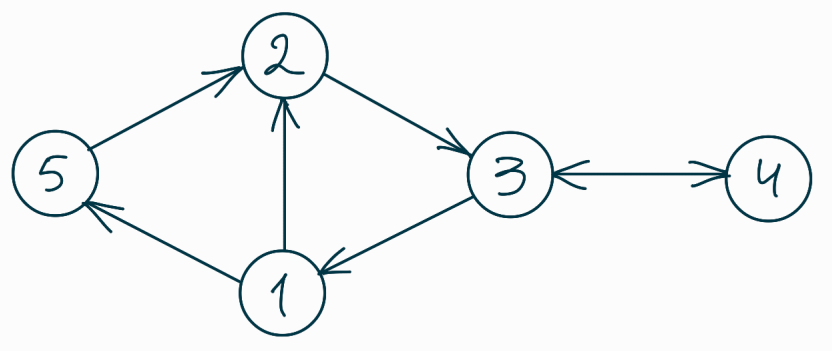
\includegraphics[width=0.35\textwidth]{images/6pic.png}
	\captionof*{figure}{Схема доказательства}
\end{center}